\begin{minipage}{.3\textwidth}
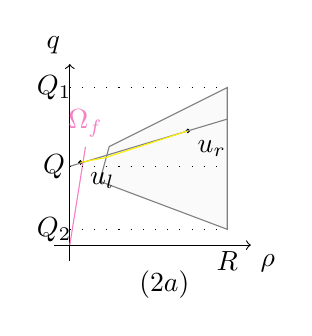
\begin{tikzpicture}
% coordinates
    \filldraw[fill=black!2, draw=black!50] plot [tension = 1] coordinates { (0.5,1.25) (2,2) (2,0.2) (0.38, 0.81) (0.5,1.25)};
    \draw[->] (0,-0.2) -- (0,2.3) node[anchor=south east] {$q$};
    %\draw[red!50, domain=0:0.7]  plot[id=x] function{x*(3*x+1)}  node[above] {$v_c(\rho)$};
    \draw[magenta!50] (0,0) -- (0.2,1.25) node[anchor = south] {$\Omega_f$};
    %\node[magenta!50] at (0.3,2.5) {$V_f$};
    \filldraw[black] (0.135,1.05) circle (0.6pt) node[anchor = north west]{$u_l$} ;
    %\filldraw[black] (0.45,1.11) circle (0.6pt) node[anchor = north west]{$u_m$} ;
    \filldraw[black] (1.5,1.45) circle (0.6pt) node[anchor = north west]{$u_r$} ;
    % \node at (1,1) {$\Omega_c$};
     \draw[->] (-0.2,0) -- (2.3,0) node[anchor=north west] {$\rho$};
     \draw[-][black!50] (0, 1) -- (2, 1.6) ;
    \node at (2,-0.2) {$R$};
     \node at (-0.2,2) {$Q_1$};
     \node at (-0.2,0.2) {$Q_2$};
     \node at (-0.2,1) {$Q$};
     \draw[loosely dotted] (0,1) -- (2,1);
     \draw[loosely dotted] (0,2) -- (2,2);
     \draw[loosely dotted] (0,0.2) -- (2,0.2);
     \node at (1.2,-0.5) {$(2a)$};
     % rarefactions and shocks
    %\draw[lime] (1.05, 1.33) -- (2, 1.6) ;
    %\draw[<-][cyan!50] (0.42, 1.19) -- (1, 1.33) ;
    
    %\draw[->][lime] (1.48,0.4)  -- (2, 0.2) ;
    \draw[-][yellow] (0.45,1.11) -- (1.5,1.45)  ;
    \draw[yellow] (0.135,1.05) -- (0.45,1.11);
    %middlepoints
     %\filldraw[black] (0.9, 0.6) circle (0.5pt) node[anchor = north]{$u_m$} ;
     %\filldraw[black] (1.48,0.4) circle (0.5pt) node[anchor =  west]{$u_r$} ;
    %endpoints
    %\filldraw[black] (1.05,1.33) circle (0.5pt) node[anchor = south east]{$u_r^1$} ;
    %\filldraw[black] (1.55,0.56) circle (0.5pt) node[anchor = south west]{$u_r^2$} ;
    
    % contacts
    %\draw[ orange!50, domain=0:1.86]  plot[id=x] function{(x/1.38)*(2-1.38)/(2-x)*0.33};
    %\draw[ orange!50, domain=0:1.28]  plot[id=x] function{(x/1.16)*(2-1.16)/(2-x)*1.63};
     
\end{tikzpicture}
\end{minipage}
\quad \quad \quad 
\begin{minipage}{.3\textwidth}
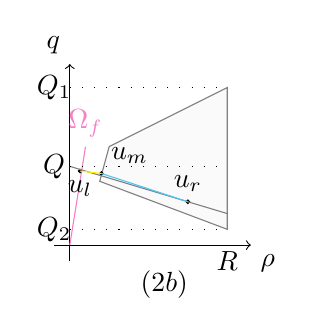
\begin{tikzpicture}
% coordinates
    \filldraw[fill=black!2, draw=black!50] plot [tension = 1] coordinates { (0.5,1.25) (2,2) (2,0.2) (0.38, 0.81) (0.5,1.25)};
    \draw[->] (0,-0.2) -- (0,2.3) node[anchor=south east] {$q$};
    %\draw[red!50, domain=0:0.7]  plot[id=x] function{x*(3*x+1)}  node[above] {$v_c(\rho)$};
    \draw[magenta!50] (0,0) -- (0.2,1.25) node[anchor = south] {$\Omega_f$};
    %\node[magenta!50] at (0.3,2.5) {$V_f$};
    \filldraw[black] (0.13,0.94) circle (0.6pt) node[anchor = north]{$u_l$} ;
    \filldraw[black] (1.5,0.55) circle (0.6pt) node[anchor = south ]{$u_r$} ;
    \filldraw[black] (0.4,0.91) circle (0.6pt) node[anchor = south west]{$u_m$} ;
    \draw[-][black!50] (0, 1) -- (2, 0.4) ;
    % \node at (1,1) {$\Omega_c$};
     \draw[->] (-0.2,0) -- (2.3,0) node[anchor=north west] {$\rho$};
    \node at (2,-0.2) {$R$};
     \node at (-0.2,2) {$Q_1$};
     \node at (-0.2,0.2) {$Q_2$};
     \node at (-0.2,1) {$Q$};
     \draw[loosely dotted] (0,1) -- (2,1);
     \draw[loosely dotted] (0,2) -- (2,2);
     \draw[loosely dotted] (0,0.2) -- (2,0.2);
     \node at (1.2,-0.5) {$(2b)$};
     % rarefactions and shocks
    %\draw[lime] (1.05, 1.33) -- (2, 1.6) ;
    %\draw[<-][cyan!50] (0.42, 1.19) -- (1, 1.33) ;
    
    \draw[-][cyan!70] (1.5,0.55)  -- (0.4,0.91) ;
    %\draw[-][cyan!50] (0.37, 0.83) -- (1.48,0.4)  ;
    \draw[yellow] (0.13,0.94) -- (0.4,0.91);
    %middlepoints
     %\filldraw[black] (0.9, 0.6) circle (0.5pt) node[anchor = north]{$u_m$} ;
     %\filldraw[black] (1.48,0.4) circle (0.5pt) node[anchor =  west]{$u_r$} ;
    %endpoints
    %\filldraw[black] (1.05,1.33) circle (0.5pt) node[anchor = south east]{$u_r^1$} ;
    %\filldraw[black] (1.55,0.56) circle (0.5pt) node[anchor = south west]{$u_r^2$} ;
    
    % contacts
    %\draw[ orange!50, domain=0:1.86]  plot[id=x] function{(x/1.38)*(2-1.38)/(2-x)*0.33};
    %\draw[ orange!50, domain=0:1.28]  plot[id=x] function{(x/1.16)*(2-1.16)/(2-x)*1.63};
     
\end{tikzpicture}
\end{minipage}